\chapter{Metodología}\label{chap:metodologia}

Este capítulo describe el procedimiento completo que transforma el corpus de reseñas
REST-MEX en un sistema de recomendación híbrido evaluable. El recorrido sigue el orden
en que se ejecuta la canalización. Primero se divide el conjunto de trabajo en
particiones de entrenamiento y prueba mediante un esquema temporal por usuario que
reproduce la situación real de predecir el siguiente destino (Sección~\ref{sec:split}).
Sobre la partición de entrenamiento se aplica la canalización de análisis de sentimientos
basado en aspectos, que segmenta cada reseña y le asigna pares aspecto-sentimiento con dos
modelos Transformer (Sección~\ref{sec:absa}). La salida aumentada con esta información se
agrega en las tres matrices estructurales $\mathbf{A}$, $\mathbf{X}$ e $\mathbf{Y}$, cuya
construcción retoma el modelo de factores explícitos del marco teórico y la ajusta con un
estudio de ablación (Sección~\ref{sec:matrices}). A partir de esas matrices se ajustan los
tres modelos individuales y se evalúan con métricas de relevancia, diversidad y cobertura
(Sección~\ref{sec:modelos}). Por último, los dos modelos basados en aspectos se combinan en
un híbrido de un solo parámetro cuyo barrido traza el compromiso entre relevancia y
cobertura que da título a este trabajo (Sección~\ref{sec:hibrido}).

% ============================================================
\section{Partición del conjunto de datos}\label{sec:split}

La evaluación de un sistema de recomendación debe estimar su capacidad para anticipar
interacciones futuras, no para reconstruir interacciones ya observadas. Una partición
aleatoria de las reseñas viola este principio, pues permitiría que el modelo aprendiera de
visitas posteriores a las que pretende predecir. Por ello se adopta una partición temporal
por usuario, conocida como \textit{last-month-out}, que reserva para prueba la actividad más
reciente de cada viajero y entrena con la anterior.

El procedimiento opera a nivel de par usuario-pueblo. Para cada usuario y cada Pueblo Mágico
que ha reseñado se determina la primera fecha de estancia, tomada como el momento en que el
usuario conoció ese destino. El mes de calendario de la estancia más reciente entre todos sus
pueblos define su último mes activo. Los pueblos cuya primera visita cae en ese último mes se
asignan al conjunto de prueba y constituyen el objetivo a predecir, mientras que el resto de
sus pueblos forman su historial de entrenamiento. Los usuarios cuyos pueblos se concentran en
su totalidad en un único mes quedan sin historial previo y se excluyen de ambas particiones,
ya que no aportan señal de entrenamiento ni permiten una evaluación honesta. Sus reseñas se
conservan por separado únicamente con fines de auditoría.

Aplicado al conjunto de trabajo de 9,582 usuarios, el esquema excluye a 448 usuarios sin
historial previo y deja 9,134 usuarios con presencia simultánea en entrenamiento y prueba. La
partición resultante reserva en promedio el 28.6\% de los pueblos de cada usuario para prueba y
el 71.4\% para entrenamiento, una proporción cercana al habitual reparto 70-30 pese a no
haberse fijado de antemano, sino haber emergido de la dinámica temporal de las visitas.

Las Figuras~\ref{fig:split_fraction} y~\ref{fig:split_count} caracterizan la partición desde
la perspectiva del usuario. La distribución de la fracción de pueblos enviados a prueba se
concentra en valores moderados, con una mediana de 0.333 y una media de 0.286: en el caso
típico, un tercio de los destinos de un usuario constituye su objetivo de prueba y los dos
tercios restantes alimentan su perfil. La masa de la distribución se ubica por debajo de la
mitad, lo que confirma que la mayoría de los usuarios conserva suficiente historial para que
los modelos colaborativo y de contenido dispongan de evidencia sobre sus preferencias. En
términos absolutos, la partición es deliberadamente exigente: la mediana es de un solo pueblo
en prueba por usuario y la media de 1.12, con un máximo de siete. La fuerte asimetría hacia la
izquierda, visible en la escala logarítmica de la Figura~\ref{fig:split_count}, refleja que
para la mayor parte de los usuarios el sistema debe acertar un único destino dentro de un
catálogo de 48 pueblos, lo que fija un listón alto para las métricas de relevancia reportadas
más adelante.

\begin{figure}[ht]
	\centering
	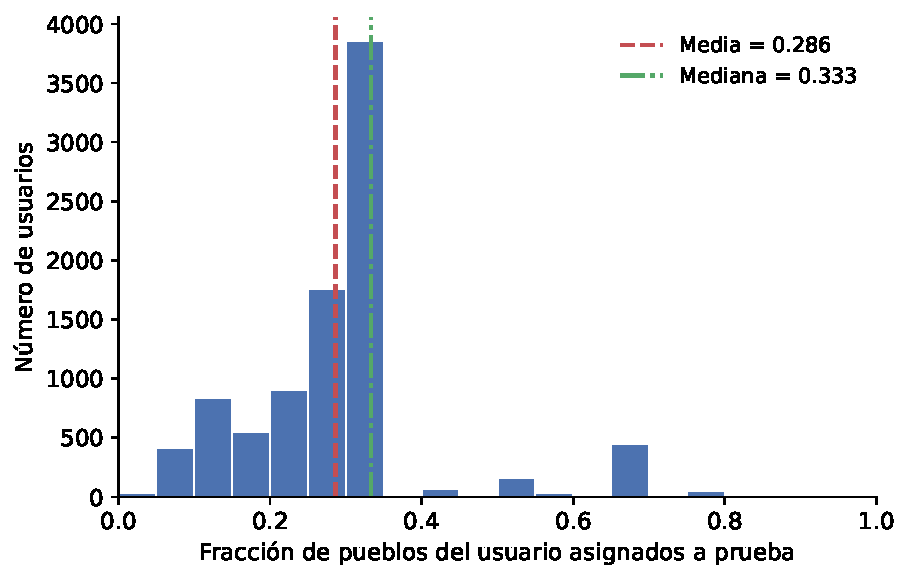
\includegraphics[width=0.7\textwidth]{figures/split_test_fraction.pdf}
	\caption[Fracción de pueblos por usuario asignada a prueba]{Distribución del número de
		usuarios según la fracción de sus pueblos visitados que la partición
		\textit{last-month-out} asigna al conjunto de prueba. Las líneas verticales señalan la
		media (0.286) y la mediana (0.333).}
	\label{fig:split_fraction}
\end{figure}

\begin{figure}[ht]
	\centering
	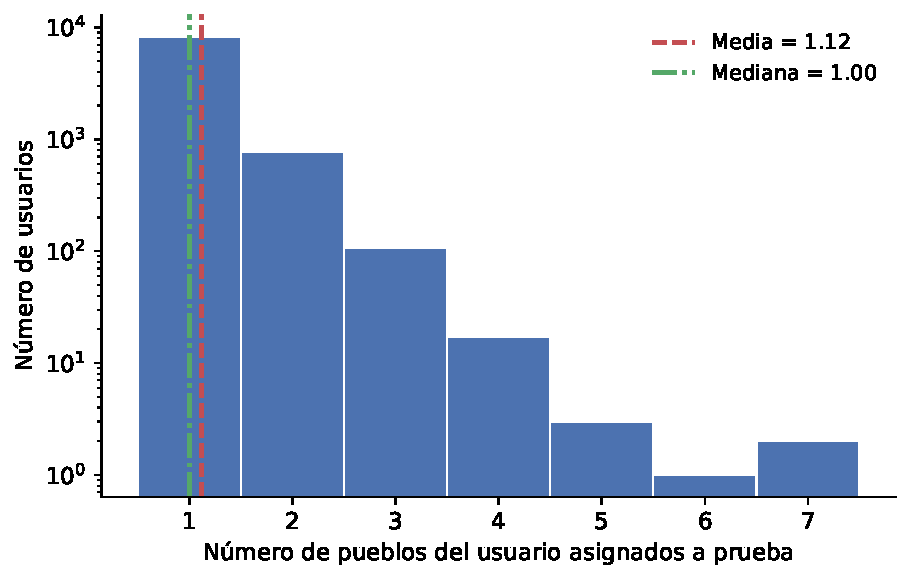
\includegraphics[width=0.7\textwidth]{figures/split_test_count.pdf}
	\caption[Número de pueblos por usuario asignado a prueba]{Distribución del número de
		usuarios según la cantidad de pueblos asignados al conjunto de prueba (eje vertical en
		escala logarítmica). La media es de 1.12 pueblos y la mediana de un solo pueblo.}
	\label{fig:split_count}
\end{figure}

% ============================================================
\section{Canalización de análisis basado en aspectos}\label{sec:absa}

El componente textual del sistema convierte cada reseña en un conjunto de pares
aspecto-sentimiento que indican qué atributos del establecimiento menciona el usuario y con qué
polaridad los valora. La Figura~\ref{fig:absa_pipeline} resume la canalización, que se aplica
exclusivamente sobre la partición de entrenamiento para evitar cualquier filtración de
información hacia el conjunto de prueba.

\begin{figure}[ht]
	\centering
	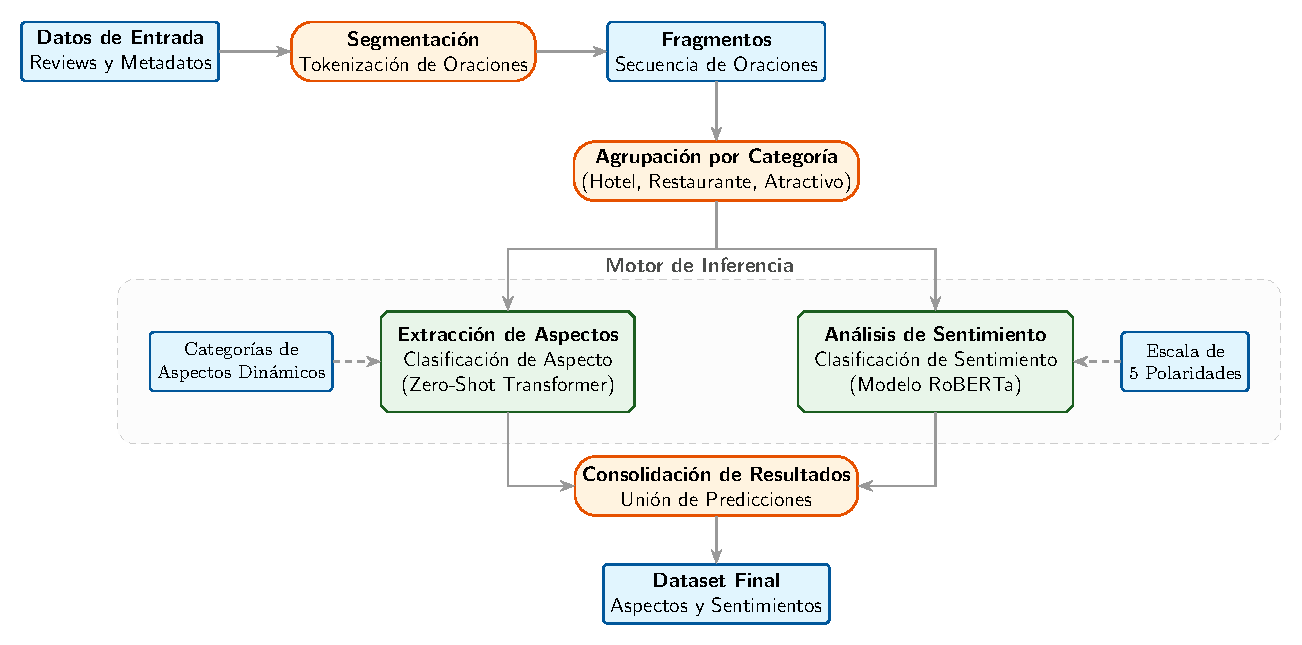
\includegraphics[width=0.85\textwidth]{figures/absa_pipeline.pdf}
	\caption[Canalización de análisis basado en aspectos]{Canalización ABSA. Cada reseña se
		segmenta en fragmentos con el segmentador Punkt; sobre cada fragmento se aplican un
		clasificador de aspecto por inferencia textual y un clasificador de sentimiento de cinco
		clases. La salida es una tabla con un par aspecto-sentimiento por fila.}
	\label{fig:absa_pipeline}
\end{figure}

\subsection*{Segmentación en fragmentos}

La unidad de análisis no es la reseña completa sino el fragmento, porque una misma reseña suele
emitir juicios de polaridad opuesta sobre aspectos distintos que conviene separar antes de
clasificar. La segmentación emplea el algoritmo no supervisado Punkt \citep{kiss_unsupervised_2006},
descrito en la Sección~\ref{subsec:sbd}, que detecta fronteras de oración a partir de
regularidades distribucionales del propio corpus sin requerir anotación manual. Su elección
frente a una segmentación ingenua por longitud fija de caracteres no es arbitraria, sino el
resultado de un análisis comparativo que se discute más abajo. Cada reseña produce así una
secuencia de fragmentos; aquellos más cortos que un umbral mínimo se descartan por carecer de
contenido evaluable, y los excepcionalmente largos se subdividen para no exceder la ventana de
los clasificadores.

\subsection*{Clasificación de aspecto y de sentimiento}

Sobre cada fragmento operan dos modelos Transformer independientes. El primero infiere el
aspecto tratado mediante clasificación \textit{zero-shot} formulada como inferencia textual
(Sección~\ref{subsec:zero_shot}). Cada aspecto candidato se transforma en una hipótesis con la
plantilla ``Esta reseña trata sobre $\langle$aspecto$\rangle$.'' y el modelo, un codificador
en español ajustado a una tarea de inferencia, estima la probabilidad de implicación entre el
fragmento y cada hipótesis \citep{yin_benchmarking_2019}. El esquema es multietiqueta: un
fragmento puede activar más de un aspecto si supera el umbral de confianza, lo que captura
oraciones que valoran simultáneamente, por ejemplo, el servicio y el precio. El conjunto de
aspectos candidatos se condiciona al tipo de establecimiento, de modo que solo se evalúan
atributos pertinentes para cada categoría. Los restaurantes admiten servicio, precio, ambiente
y comida; los hoteles añaden ubicación y habitación; y los atractivos sustituyen estos últimos
por naturaleza y cultura. La unión de todas las categorías produce los ocho aspectos sobre los
que se construirán después las matrices.

El segundo modelo asigna la polaridad del fragmento sobre una escala ordinal de cinco niveles,
de Muy Negativo a Muy Positivo (Sección~\ref{subsec:sentiment_models}). Se trata de un RoBERTa
en español preentrenado sobre la Biblioteca Nacional de España y posteriormente adaptado al
dominio turístico \citep{liu2019roberta}, lo que alinea la granularidad de la predicción con la
escala de calificación de una a cinco estrellas del propio corpus. La salida de la canalización
es una tabla en la que cada fila corresponde a un par aspecto-sentimiento, acompañado de la
confianza de ambos clasificadores, junto con los identificadores de usuario, pueblo, lugar y
tipo necesarios para la agregación posterior.

\subsection*{Selección del segmentador}

La decisión de segmentar con Punkt en lugar de partir el texto en bloques de longitud fija se
sustenta en un estudio comparativo sobre el conjunto completo de reseñas, resumido en la
Tabla~\ref{tab:punkt_vs_char}. La segmentación por caracteres genera más fragmentos (322,885
frente a 230,006) porque corta el texto a ciegas, sin respetar las fronteras lingüísticas, lo
que produce unidades que parten oraciones por la mitad. El efecto sobre los clasificadores es
asimétrico. La confianza mediana del clasificador de aspecto apenas cambia entre ambas
estrategias, en torno a 0.48, pero la del clasificador de sentimiento cae de 0.843 con Punkt a
0.727 con el corte fijo. La explicación es que la polaridad depende críticamente del contexto
local de la oración, que el corte por caracteres fragmenta, mientras que la detección de aspecto
se apoya en palabras clave que sobreviven a la fragmentación. Dado que Punkt conserva la
coherencia sintáctica con un número menor de fragmentos y mejora la confianza de la subtarea más
sensible al contexto, se adopta como segmentador definitivo.

\begin{table}[ht]
	\centering
	\caption{Comparación entre la segmentación por oraciones (Punkt) y por bloques de
		caracteres de longitud fija, sobre el conjunto completo de reseñas.}
	\label{tab:punkt_vs_char}
	\begin{tabular}{lrr}
		\toprule
		\textbf{Métrica}                       & \textbf{Punkt} & \textbf{Caracteres} \\
		\midrule
		Fragmentos generados                   & 230,006        & 322,885             \\
		Fragmentos por reseña (media)          & 3.71           & 4.07                \\
		Longitud del fragmento (mediana, car.) & 75             & 100                 \\
		Confianza de aspecto (mediana)         & 0.483          & 0.480               \\
		Confianza de sentimiento (mediana)     & 0.843          & 0.727               \\
		\bottomrule
	\end{tabular}
\end{table}

La Figura~\ref{fig:absa_confidence} muestra la distribución de la confianza de ambos
clasificadores sobre la salida definitiva. El contraste entre los dos paneles revela una
asimetría informativa relevante. La confianza de sentimiento se acumula cerca de la unidad, con
mediana 0.843, lo que indica que el modelo adaptado al dominio resuelve la polaridad con poca
ambigüedad. La confianza de aspecto, en cambio, se reparte de forma mucho más extendida y se
centra en torno a 0.483, reflejo de que la detección de aspecto en modo \textit{zero-shot} es la
subtarea intrínsecamente más difícil: opera sin ejemplos etiquetados, debe discriminar entre
categorías semánticamente próximas y admite fragmentos que no tratan con claridad ninguno de los
aspectos candidatos. Esta brecha justifica el filtrado por umbral de confianza en la detección de
aspecto y anticipa que la señal de aspecto, más ruidosa, conviene agregarla por volumen antes de
incorporarla a las matrices.

\begin{figure}[ht]
	\centering
	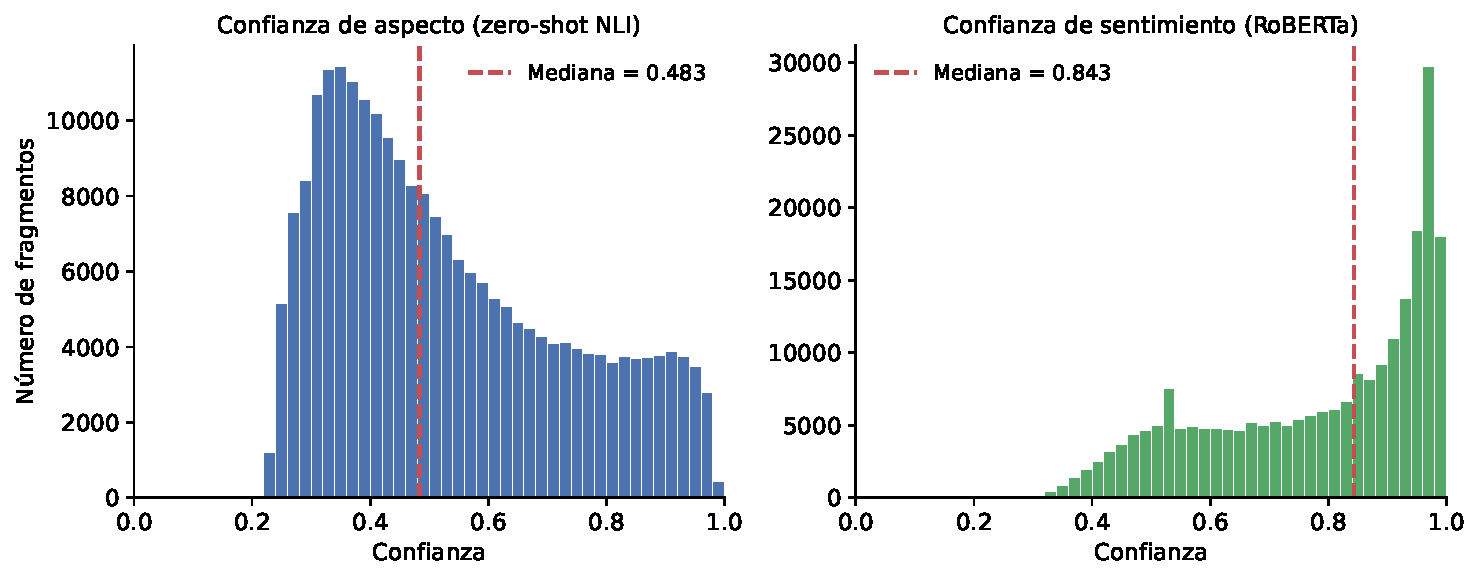
\includegraphics[width=\textwidth]{figures/absa_confidence.pdf}
	\caption[Confianza de los clasificadores de aspecto y sentimiento]{Distribución de la
		confianza del clasificador de aspecto (izquierda) y del clasificador de sentimiento
		(derecha) sobre los fragmentos de la partición de entrenamiento. La línea discontinua
		marca la mediana de cada distribución.}
	\label{fig:absa_confidence}
\end{figure}

Finalmente, la Figura~\ref{fig:aspect_tipo} confirma que el condicionamiento de los aspectos por
tipo de establecimiento se traduce en perfiles coherentes con el dominio. Los aspectos exclusivos
de cada categoría aparecen únicamente donde corresponde: la habitación y la ubicación se
concentran en los hoteles, la comida en los restaurantes, y la naturaleza y la cultura en los
atractivos turísticos, mientras que los aspectos transversales como el servicio y el ambiente se
distribuyen entre las tres categorías. Esta coherencia valida que la canalización captura
estructura semántica de dominio y no simplemente ruido.

\begin{figure}[ht]
	\centering
	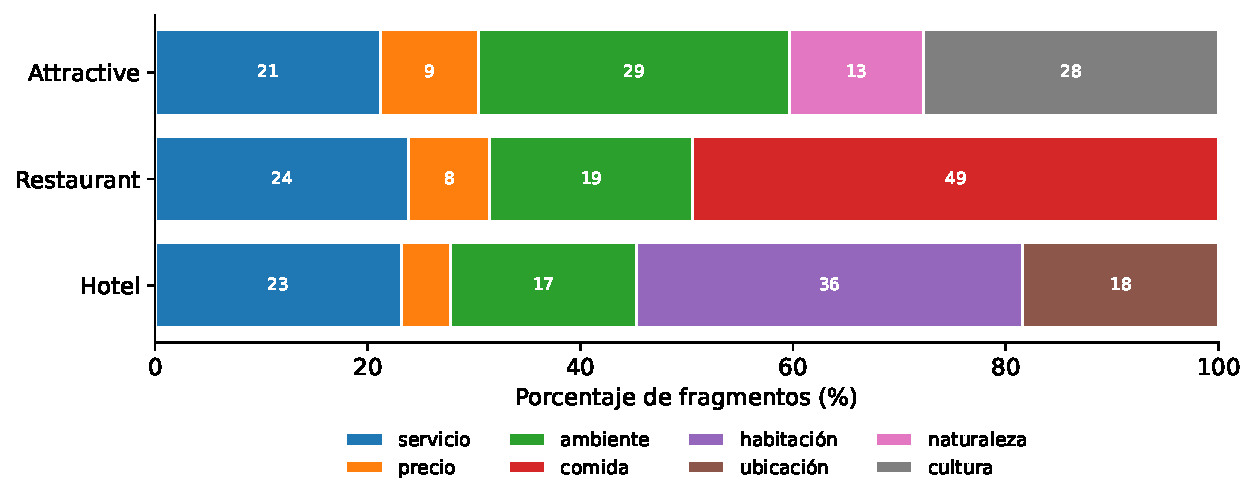
\includegraphics[width=0.9\textwidth]{figures/absa_aspect_by_tipo.pdf}
	\caption[Composición de aspectos por tipo de establecimiento]{Porcentaje de fragmentos por
		aspecto dentro de cada tipo de establecimiento. Los aspectos específicos de cada categoría
		aparecen solo donde son pertinentes, lo que evidencia el condicionamiento por tipo.}
	\label{fig:aspect_tipo}
\end{figure}

% ============================================================
\section{Construcción de las matrices estructurales}\label{sec:matrices}

La información extraída por la canalización ABSA se agrega en tres matrices que constituyen la
entrada común de todos los modelos. La matriz de calificaciones $\mathbf{A}$ resume la señal
numérica de las interacciones, mientras que las matrices de atención del usuario $\mathbf{X}$ y
de calidad del pueblo $\mathbf{Y}$ codifican las preferencias y las cualidades en el espacio de
aspectos, siguiendo el modelo de factores explícitos de \citet{zhang_explicit_2014} presentado
en la Sección~\ref{sec:absa_rs}.

\subsection*{Matriz de calificaciones}

La matriz $\mathbf{A} \in \mathbb{R}^{|\mathcal{U}| \times |\mathcal{I}|}$ recoge la valoración
global de cada usuario sobre cada pueblo. Su entrada es el promedio de las calificaciones que el
usuario otorgó a los establecimientos del pueblo,
\begin{equation}\label{eq:matrix_A}
	A_{u,p} = \frac{1}{|\mathcal{R}_{u,p}|} \sum_{r \in \mathcal{R}_{u,p}} \text{calif}(r),
\end{equation}
donde $\mathcal{R}_{u,p}$ es el conjunto de reseñas del usuario $u$ en el pueblo $p$. Las
entradas correspondientes a pares no observados quedan vacías, lo que refleja la elevada
dispersión del corpus (90.32\% de celdas sin observar) y delimita el universo de candidatos sobre
el que opera la recomendación.

\subsection*{Matrices de aspectos}

La matriz de atención del usuario $\mathbf{X} \in \mathbb{R}^{|\mathcal{U}| \times |\mathcal{A}|}$
mide la importancia que cada usuario concede a cada aspecto a partir de la frecuencia con que lo
menciona. Siguiendo la forma sigmoidal de la Ecuación~(\ref{eq:efm_X}), pero introduciendo un
factor de escala $T_x$, se define
\begin{equation}\label{eq:matrix_X}
	X_{u,a} = 1 + (N - 1) \left( \frac{2}{1 + \exp(-t_{u,a} / T_x)} - 1 \right),
\end{equation}
donde $t_{u,a}$ es el número de fragmentos en que el usuario $u$ menciona el aspecto $a$, $N=5$
es el extremo superior de la escala y $T_x$ es la mediana de los conteos no nulos. El factor
$T_x$ sitúa el punto de inflexión de la sigmoide en la frecuencia típica de mención, de modo que
la importancia discrimina entre usuarios en el rango de conteos efectivamente observado en lugar
de saturarse.

La matriz de calidad del pueblo $\mathbf{Y} \in \mathbb{R}^{|\mathcal{I}| \times |\mathcal{A}|}$
combina la polaridad media de la comunidad sobre cada aspecto con el volumen de menciones que la
respalda. Partiendo de la Ecuación~(\ref{eq:efm_Y}) y aplicando el mismo escalamiento,
\begin{equation}\label{eq:matrix_Y}
	Y_{p,a} = 1 + \frac{N - 1}{1 + \exp\!\left(-\, t_{p,a}\, s_{p,a} / T_y \right)},
\end{equation}
donde $s_{p,a} \in [-1, 1]$ es el sentimiento medio sobre el aspecto $a$ en el pueblo $p$
(obtenido al centrar y normalizar la escala de cinco clases), $t_{p,a}$ es el número de menciones
que lo sustentan y $T_y$ es la mediana de la magnitud no nula del producto $t_{p,a}\, s_{p,a}$.
El producto sentimiento por volumen otorga más peso a una valoración positiva sostenida por
muchas opiniones que a un juicio aislado, en línea con la intuición del modelo original.

\subsection*{Estudio de ablación}

La transcripción literal de las Ecuaciones~(\ref{eq:efm_X}) y~(\ref{eq:efm_Y}) introduce el
conteo de menciones $t$ directamente en el argumento de la sigmoide. En el corpus REST-MEX, donde
un pueblo popular acumula cientos de menciones por aspecto, este conteo crece sin cota y satura la
sigmoide: casi todas las entradas de $\mathbf{Y}$ se aproximan a su máximo y la matriz pierde
capacidad de discriminación. El factor de escala $T$ que aparece en las
Ecuaciones~(\ref{eq:matrix_X}) y~(\ref{eq:matrix_Y}) corrige precisamente este efecto al
normalizar la señal por su magnitud típica. Para verificar que este ajuste es necesario y
suficiente se diseñó un estudio de ablación que cruza dos decisiones sobre la construcción de las
matrices: incorporar o no el escalamiento $T$, y ponderar o no el volumen mediante una compresión
logarítmica adicional. La Tabla~\ref{tab:ablation} reporta las cuatro variantes resultantes,
evaluadas con el modelo de contenido a $K=10$.

\begin{table}[ht]
	\centering
	\caption{Ablación de la construcción de $\mathbf{X}$ e $\mathbf{Y}$. La columna de saturación
		indica la fracción de entradas de $\mathbf{Y}$ que superan 4.5 sobre un máximo de 5.
		Resultados del modelo de contenido a $K=10$.}
	\label{tab:ablation}
	\begin{tabular}{clccc}
		\toprule
		\textbf{Variante} & \textbf{Construcción de $\mathbf{Y}$}         & \textbf{$\mathbf{Y}$ saturada} & \textbf{NDCG@10} & \textbf{Cov@10} \\
		\midrule
		A                 & volumen logarítmico $+\,T$                    & 0.013                          & 0.388            & 0.958           \\
		B                 & forma literal de Zhang (sin $T$)              & 0.979                          & 0.324            & 0.896           \\
		C                 & escalamiento $T$ (sin logaritmo), $X$ literal & 0.336                          & 0.418            & 0.958           \\
		D                 & escalamiento $T$ (sin logaritmo)              & 0.336                          & 0.418            & 0.958           \\
		\bottomrule
	\end{tabular}
\end{table}

Los resultados son concluyentes. La variante B, que reproduce la forma literal del modelo de
factores explícitos sin escalamiento, satura el 97.9\% de las entradas de $\mathbf{Y}$ por encima
de 4.5 y colapsa su varianza por fila, lo que la convierte en la peor configuración con un NDCG@10
de apenas 0.324. Introducir el escalamiento $T$ (variantes C y D) reduce la saturación a un tercio
de las entradas y recupera la capacidad de discriminación, con una ganancia cercana a nueve puntos
de NDCG y seis de cobertura respecto de B. La compresión logarítmica del volumen (variante A)
también evita la saturación, pero lo hace en exceso: comprime tanto la señal que rebaja el NDCG a
0.388, por debajo de las variantes que solo escalan con $T$. La comparación entre C y D, idénticas
salvo en la construcción de $\mathbf{X}$, muestra además que aplicar el mismo escalamiento a la
matriz del usuario evita que los aspectos muy frecuentes saturen su importancia. Se adopta por
tanto la variante D, que conserva únicamente el término de escalamiento $T$ en ambas matrices y
descarta la ponderación logarítmica, tal como recogen las Ecuaciones~(\ref{eq:matrix_X})
y~(\ref{eq:matrix_Y}).

% ============================================================
\section{Modelos de recomendación}\label{sec:modelos}

A partir de las tres matrices se ajustan tres modelos individuales que cubren las dos grandes
familias de la recomendación. El primero es un filtrado colaborativo clásico que opera sobre las
calificaciones; los otros dos explotan las representaciones de aspectos, uno por la vía
colaborativa y otro por la vía de contenido. Todos generan una lista de los $K$ pueblos no
visitados con mayor puntuación predicha, y se evalúan con las métricas de relevancia, diversidad
y cobertura definidas en la Sección~\ref{subsec:evaluation}, tomando como verdad de referencia los
pueblos que cada usuario reservó para prueba.

\paragraph{CFClassic.} Es la factorización matricial con sesgos descrita por la
Ecuación~(\ref{eq:svd_bias}) \citep{koren_matrix_2009}. Predice la calificación como
$\hat{r}_{u,p} = \mu + b_u + b_p + \mathbf{p}_u^\top \mathbf{q}_p$, donde $\mu$ es la media global,
$b_u$ y $b_p$ los sesgos de usuario y pueblo, y $\mathbf{p}_u, \mathbf{q}_p$ los vectores latentes
aprendidos por descenso de gradiente estocástico con regularización sobre las entradas observadas
de $\mathbf{A}$. Constituye la referencia colaborativa basada exclusivamente en la señal numérica
y, por construir su predicción a partir de $\mathbf{A}$, no interviene en el híbrido.

\paragraph{CFAttention.} Es un filtrado colaborativo usuario-usuario cuya novedad reside en medir
la afinidad entre usuarios en el espacio de aspectos en lugar de en el de calificaciones. La
similitud se define a partir de la distancia euclidiana entre las filas de $\mathbf{X}$,
$\text{sim}(u,v) = 1 / (1 + \lVert \mathbf{X}_u - \mathbf{X}_v \rVert_2)$, y la predicción corrige
la media del usuario con la desviación ponderada de sus vecinos más afines,
\begin{equation}\label{eq:cfattention}
	\hat{r}_{u,p} = \mu_u + \frac{\sum_{v \in \mathcal{N}_k(u)} \text{sim}(u,v)\, (A_{v,p} - \mu_v)}
	{\sum_{v \in \mathcal{N}_k(u)} |\text{sim}(u,v)|},
\end{equation}
con $\mathcal{N}_k(u)$ el conjunto de los $k$ vecinos más similares que han visitado el pueblo
$p$. De este modo las preferencias por aspecto, y no la coincidencia en calificaciones, gobiernan
la formación de la vecindad. Es la rama colaborativa del híbrido.

\paragraph{CBQuality.} Es el modelo de contenido derivado del término explícito del EFM, según la
versión normalizada de la Ecuación~(\ref{eq:cbquality}). Predice
$\hat{r}_{u,p} = \sum_{a} (X_{u,a} / \sum_{a'} X_{u,a'})\, Y_{p,a}$, esto es, el grado de
correspondencia entre la importancia que el usuario asigna a cada aspecto y la calidad del pueblo
en ese mismo aspecto, sin recurrir a ningún factor latente. Es la rama de contenido del híbrido.

La Tabla~\ref{tab:modelos} reúne el rendimiento de los tres modelos para $K \in \{5, 10, 20\}$.
El patrón es nítido y revela una complementariedad que motiva la fusión. CBQuality domina con
holgura en todas las métricas de relevancia y en todos los cortes: su NDCG@10 de 0.312 más que
duplica el de los dos modelos colaborativos, y otro tanto ocurre con la exhaustividad y el
acierto. Este resultado confirma que, bajo la fuerte dispersión del corpus, el emparejamiento de
perfiles de aspecto recupera preferencias que la escasa coincidencia de calificaciones no permite
estimar de forma fiable, en coherencia con las ventajas del filtrado de contenido ante el problema
del arranque en frío. El precio que paga CBQuality es la cobertura: a $K=5$ apenas expone el 43.8\%
del catálogo, porque tiende a concentrar sus recomendaciones en los pueblos de mayor calidad
agregada. Los dos modelos colaborativos exhiben el comportamiento opuesto, con cobertura
prácticamente total y la mayor diversidad intra-lista, pero con una relevancia muy inferior. Entre
ellos, CFAttention y CFClassic quedan próximos en relevancia, lo que indica que la ventaja de medir
la afinidad en el espacio de aspectos no se traduce por sí sola en mejor ordenamiento, aunque sí
aporta la cobertura y la diversidad que a CBQuality le faltan. Esta tensión entre relevancia y
cobertura es la que el modelo híbrido busca administrar.

\begin{table}[ht]
	\centering
	\caption{Rendimiento de los modelos individuales para distintos cortes $K$. P, R y NDCG
		denotan precisión, exhaustividad y \textit{ranking}; MRR el rango recíproco medio; ILD la
		diversidad intra-lista; y Cov la cobertura de catálogo.}
	\label{tab:modelos}
	\begin{tabular}{llrrrrrr}
		\toprule
		\textbf{Modelo} & \textbf{$K$} & \textbf{P@$K$} & \textbf{R@$K$} & \textbf{NDCG@$K$} & \textbf{MRR} & \textbf{ILD} & \textbf{Cov@$K$} \\
		\midrule
		CBQuality       & 5            & 0.083          & 0.361          & 0.260             & 0.236        & 0.000        & 0.438            \\
		                & 10           & 0.059          & 0.516          & 0.312             & 0.256        & 0.000        & 0.646            \\
		                & 20           & 0.041          & 0.735          & 0.367             & 0.271        & 0.001        & 0.958            \\
		\midrule
		CFClassic       & 5            & 0.032          & 0.143          & 0.086             & 0.071        & 0.002        & 0.979            \\
		                & 10           & 0.032          & 0.289          & 0.134             & 0.092        & 0.002        & 1.000            \\
		                & 20           & 0.031          & 0.549          & 0.201             & 0.109        & 0.002        & 1.000            \\
		\midrule
		CFAttention     & 5            & 0.029          & 0.130          & 0.080             & 0.068        & 0.006        & 0.979            \\
		                & 10           & 0.029          & 0.258          & 0.122             & 0.086        & 0.006        & 1.000            \\
		                & 20           & 0.029          & 0.518          & 0.188             & 0.104        & 0.006        & 1.000            \\
		\bottomrule
	\end{tabular}
\end{table}

Conviene precisar que CFClassic se evaluó sobre el subconjunto de usuarios de prueba presentes en
su matriz de entrenamiento, ligeramente menor al de los modelos basados en aspectos, por lo que su
comparación directa con ellos debe leerse con esa salvedad. Aun así, la conclusión cualitativa no
cambia: ninguno de los modelos colaborativos se aproxima a la relevancia del modelo de contenido.

% ============================================================
\section{Modelo híbrido y compromiso relevancia--cobertura}\label{sec:hibrido}

El análisis de los modelos individuales muestra que la relevancia y la cobertura provienen de
componentes distintos: el modelo de contenido aporta el ordenamiento certero y el colaborativo la
exposición del catálogo. El híbrido las combina mediante la fusión convexa de la
Ecuación~(\ref{eq:hybrid}), restringida a las dos ramas basadas en aspectos,
\begin{equation}\label{eq:hybrid_final}
	\hat{y}_{u,p}(\alpha) = \alpha\, \hat{y}^{\,\mathrm{CFAttention}}_{u,p} + (1 - \alpha)\, \hat{y}^{\,\mathrm{CBQuality}}_{u,p},
	\qquad \alpha \in [0, 1].
\end{equation}
Ambas ramas se ajustan una sola vez y el parámetro $\alpha$ se limita a reponderar sus
predicciones, por lo que recorrer todo el rango de fusión es computacionalmente trivial. El
extremo $\alpha = 0$ recupera el modelo de contenido puro y el extremo $\alpha = 1$ el
colaborativo, de modo que la Tabla~\ref{tab:modelos} ya contiene los dos vértices de la fusión.

La Figura~\ref{fig:alpha_sweep} traza el barrido de $\alpha$ a $K=10$. Las dos métricas se mueven
en direcciones opuestas y de forma monótona: el NDCG@10 desciende de forma continua desde 0.312 en
$\alpha=0$ hasta 0.122 en $\alpha=1$, mientras que la cobertura asciende desde 0.646 hasta
saturarse en 1.0 alrededor de $\alpha \approx 0.8$. La relevancia, por tanto, proviene de CBQuality
y la cobertura de CFAttention, y no existe un valor de $\alpha$ que maximice ambas
simultáneamente. Esta es la manifestación empírica del compromiso multiobjetivo formalizado en la
Sección~\ref{sec:moo}.

\begin{figure}[ht]
	\centering
	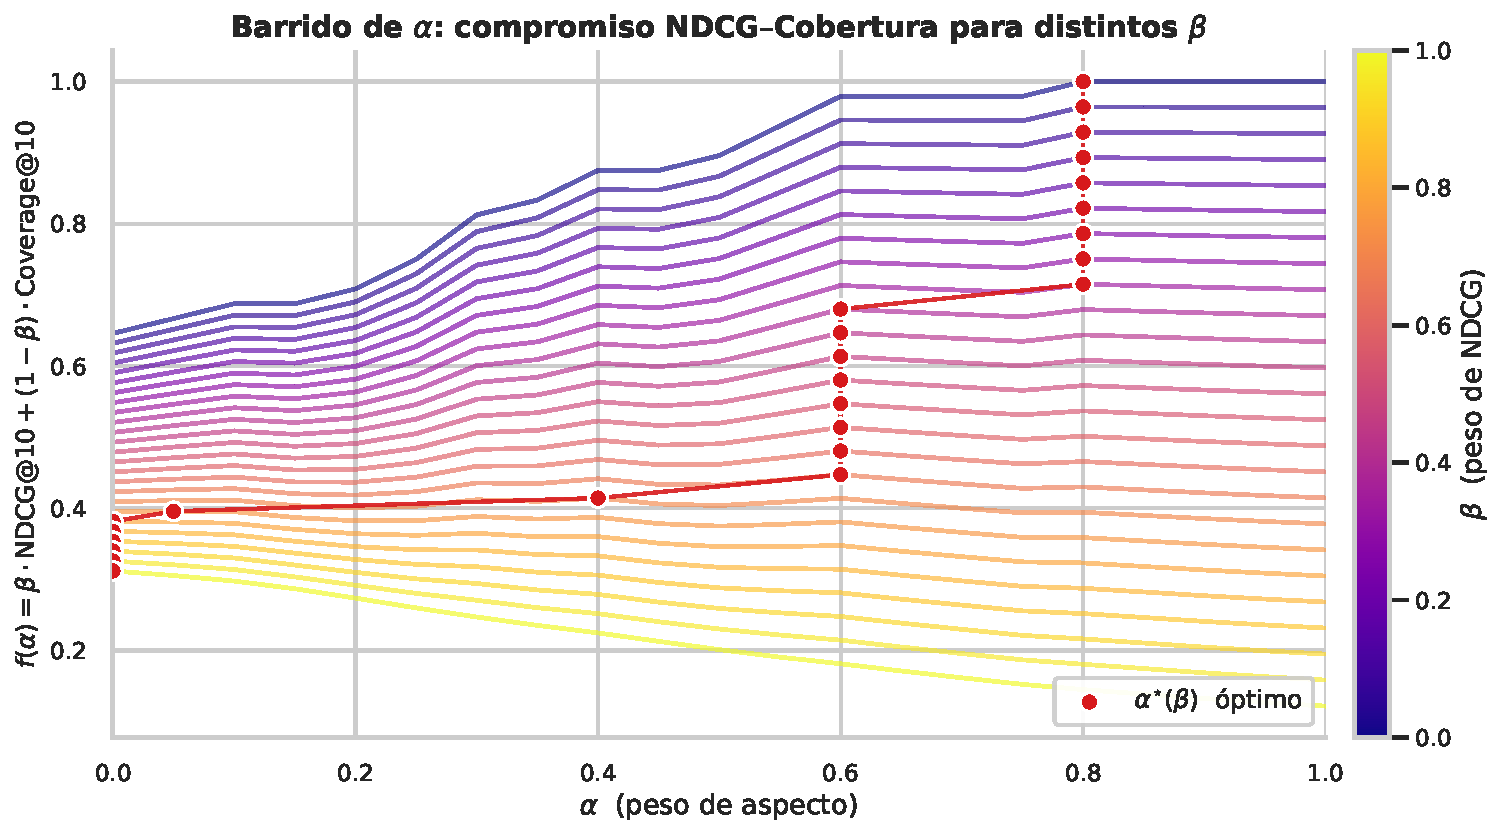
\includegraphics[width=0.72\textwidth]{figures/alpha_sweep.pdf}
	\caption[Barrido del peso de fusión]{Relevancia (NDCG@10) y cobertura (Cov@10) en función del
		peso de fusión $\alpha$. Al aumentar $\alpha$ la relevancia decrece y la cobertura crece
		hasta saturarse, lo que evidencia el conflicto entre ambos objetivos.}
	\label{fig:alpha_sweep}
\end{figure}

La selección de un único $\alpha$ se resuelve escalarizando los dos objetivos con un peso de
preferencia $\beta$, según la Ecuación~(\ref{eq:scalarization}), y leyendo el óptimo
$\alpha^{\star}(\beta)$ directamente del barrido como indica la Ecuación~(\ref{eq:alpha_star}). La
Figura~\ref{fig:alpha_vs_beta} presenta el análisis de sensibilidad resultante. A medida que la
preferencia se inclina hacia la relevancia, esto es, conforme $\beta$ crece, el óptimo migra en
escalera desde un régimen colaborativo, con $\alpha^{\star} \approx 0.8$ cuando solo importa la
cobertura, hacia el modelo de contenido puro, con $\alpha^{\star} \to 0$ cuando solo importa la
relevancia. Resulta ilustrativo que el óptimo nunca rebase $\alpha^{\star} = 0.8$: como la
cobertura ya alcanza su máximo en ese punto, cualquier incremento adicional de $\alpha$ solo
sacrificaría relevancia sin ganar cobertura, por lo que esas configuraciones quedan descartadas.

\begin{figure}[ht]
	\centering
	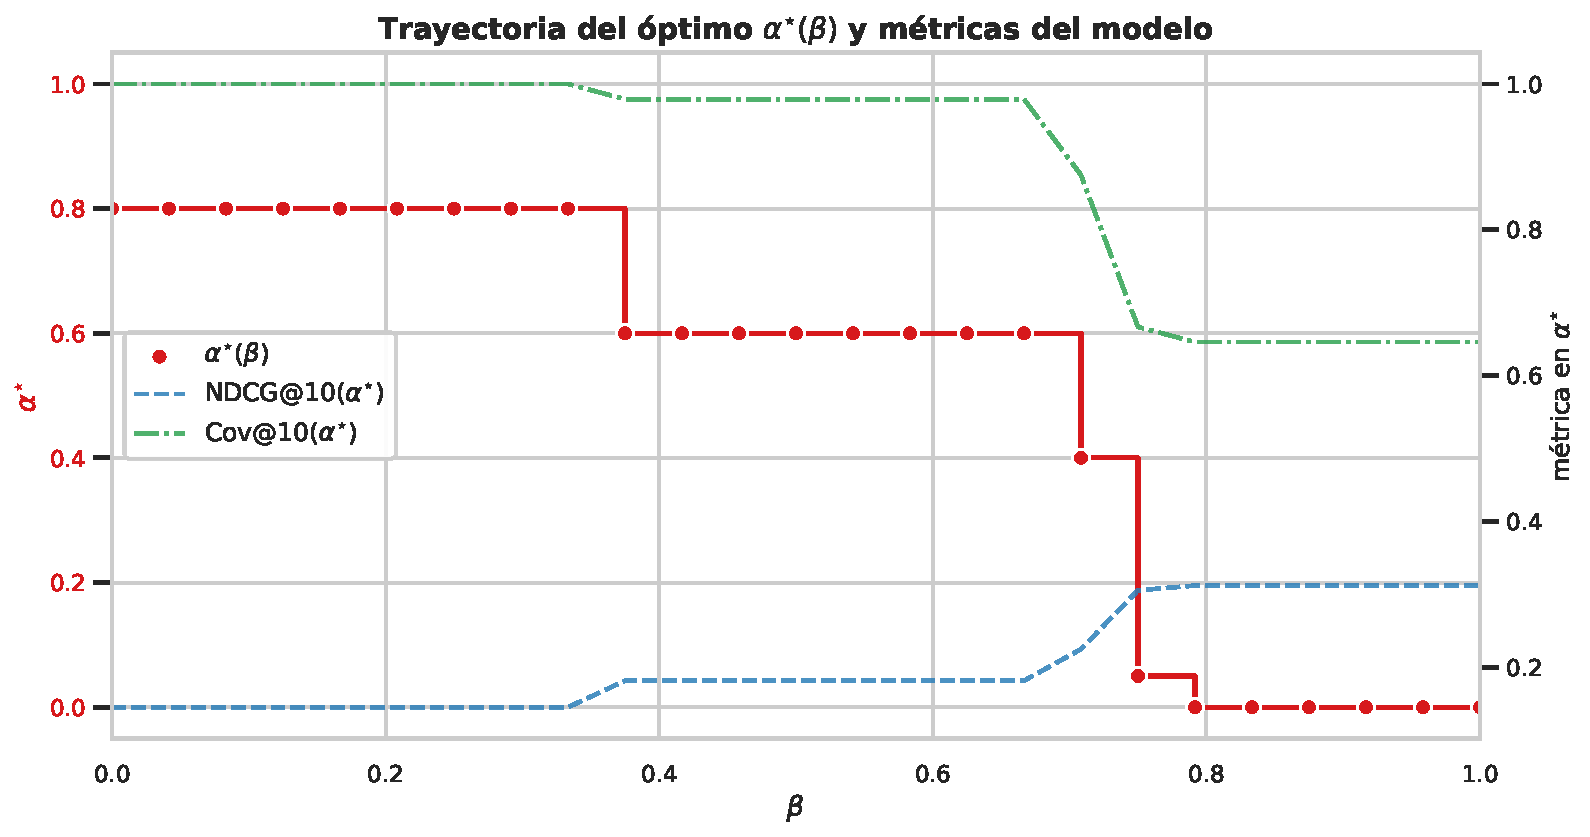
\includegraphics[width=0.75\textwidth]{figures/alphaVSbeta.pdf}
	\caption[Análisis de sensibilidad del óptimo]{Trayectoria del óptimo $\alpha^{\star}(\beta)$
		(escalera) y métricas alcanzadas en él. Al priorizar la relevancia ($\beta$ creciente) el
		óptimo se desplaza de un filtrado colaborativo a uno basado en contenido, mientras la
		cobertura cede terreno y el NDCG@10 aumenta.}
	\label{fig:alpha_vs_beta}
\end{figure}

Finalmente, la Figura~\ref{fig:pareto_realized} representa el frente de Pareto realizado del
sistema en el plano cobertura-relevancia, el análogo empírico del frente teórico de la
Figura~\ref{fig:pareto_front}. Cada punto corresponde a un valor de $\alpha$; los puntos no
dominados, que ningún otro supera a la vez en relevancia y cobertura, forman la frontera eficiente
sobre la que debe situarse cualquier elección razonable de fusión. Las configuraciones con
$\alpha > 0.8$ quedan por debajo de la frontera, dominadas por $\alpha = 0.8$, que alcanza la misma
cobertura máxima con mayor relevancia. La trayectoria $\alpha^{\star}(\beta)$ recorre esta frontera
de un extremo al otro, y la elección final del peso de fusión deja de ser una cuestión técnica para
convertirse en una decisión de diseño sobre cuánta relevancia se está dispuesto a ceder a cambio de
exponer una mayor parte del catálogo.

\begin{figure}[ht]
	\centering
	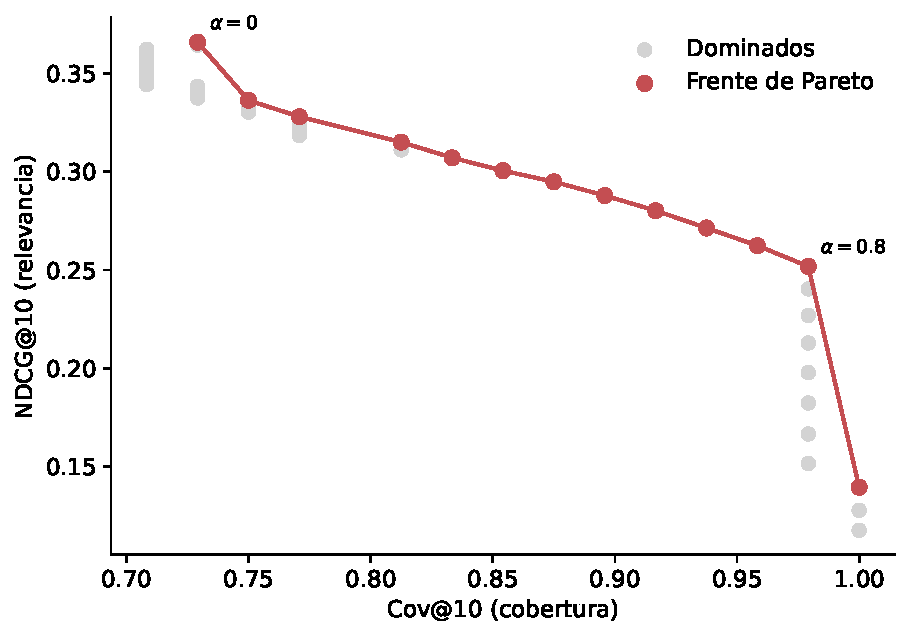
\includegraphics[width=0.68\textwidth]{figures/pareto_realized.pdf}
	\caption[Frente de Pareto realizado]{Frente de Pareto realizado del híbrido en el plano
		Cov@10--NDCG@10. Cada punto es un valor de $\alpha$; los puntos resaltados son no dominados
		y conforman la frontera eficiente. Las configuraciones con $\alpha > 0.8$ quedan dominadas
		por $\alpha = 0.8$.}
	\label{fig:pareto_realized}
\end{figure}
